\chapter{APPLICATIONS OF PLASMA-LIQUID SYSTEMS}
\label{chap:applications}

\Cref{chap:expt_opt} describes the experimental designs used to create and optimize plasma-liquid interactions. The several designs include the base case where the VHF source is pointed straight into a water reservoir, cases where water is sprayed through the plasma using either a green house sprayer or a specially designed nozzle electrode, and the final case where water is pumped through the middle of the VHF source's inner conductor to create a water layer on top of the powered electrode. Along with measuring and performing diagnostics to understand the physical and chemical nature of these systems, we can use these systems in various applications. This chapter explores two such applications. \Cref{sec:fertigation} investigates use of plasma to generate fertilizer and enhance plant growth. The latter half of the chapter studies degradation of aqueous contaminants like 1,4-dioxane and perfluorooctanesulfonic acid (PFOS) with the VHF plasma source.

\section{Fertigation}
\label{sec:fertigation}

For a published version of much of the fertigation work described below, the author encourages the interested reader to navigate to \cite{Lindsay2014}.

\subsection{Experiment}

The glow discharge used to create PAW for plant treatment is generated using the single-stub matched coaxial structure and 162 MHz power source depicted in \cref{chap:expt_opt}.  For detailed design and electrical characteristics, see \cite{byrns2012vhf}.   Delivered power to the plasma was held constant at 420 W; the air feed gas was flowed at .11 m3/min.  To generate a single "batch" of PAW, 1.9 L of distilled water was exposed to the air discharge for 72-80 minutes.  The height of the treatment container was controlled such that the discharge was held roughly .5 cm above the water surface for the duration of exposure.  Treatment time was chosen such that the final water pH was 2.7.  PAW batches were stored at acidic pH for two days and then NaHCO3 was added until a plant friendly pH of 6 was achieved. Final nitrate and nitrite concentrations were determined using ion chromatography (IC), and were between 113-120 ppm and 4-6 ppm respectively. A new batch of PAW was created once every two days in order to keep up with plant watering demand.  A representative experimental set-up for exposure of water to the glow discharge can be seen in \cref{fig:batch_scheme}.

\begin{figure}[htbp]
  \centering
  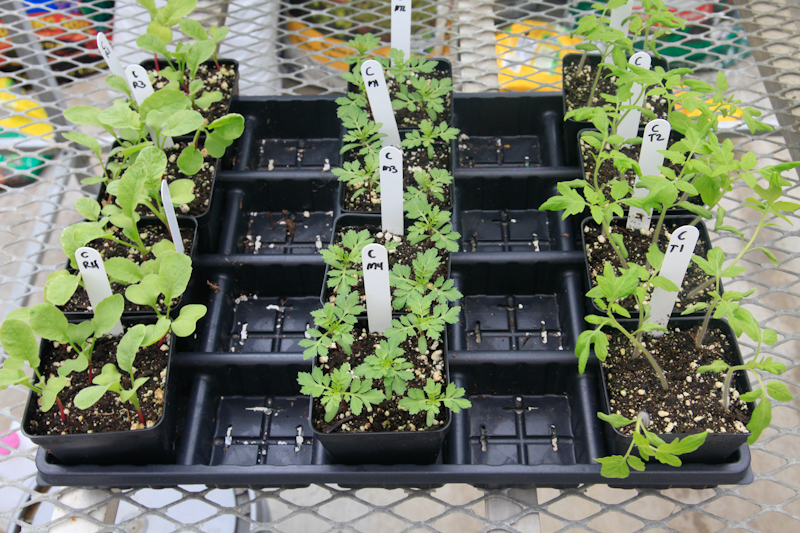
\includegraphics[width=0.9\textwidth]{Figure2_word.jpg}
  \caption{CC group potting arrangement during weeks 1 and 2 (germination phase).  Photo taken at end of week 2. For scale, each pot is 8.9 cm x 8.9 cm x 6.1 cm (length x width x height)}
  \label{fig:cc}
\end{figure}

\begin{figure}[htbp]
  \centering
  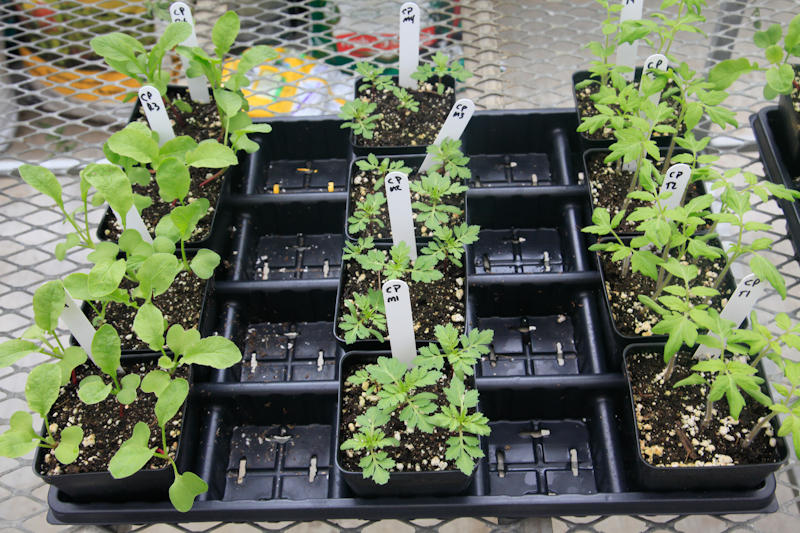
\includegraphics[width=0.9\textwidth]{Figure3_word.jpg}
  \caption{CP group potting arrangement during weeks 1 and 2 (germination phase). Photo taken at end of week 2. For scale, each pot is 8.9 cm x 8.9 cm x 6.1 cm (length x width x height)}
  \label{fig:cp}
\end{figure}

\begin{figure}[htbp]
  \centering
  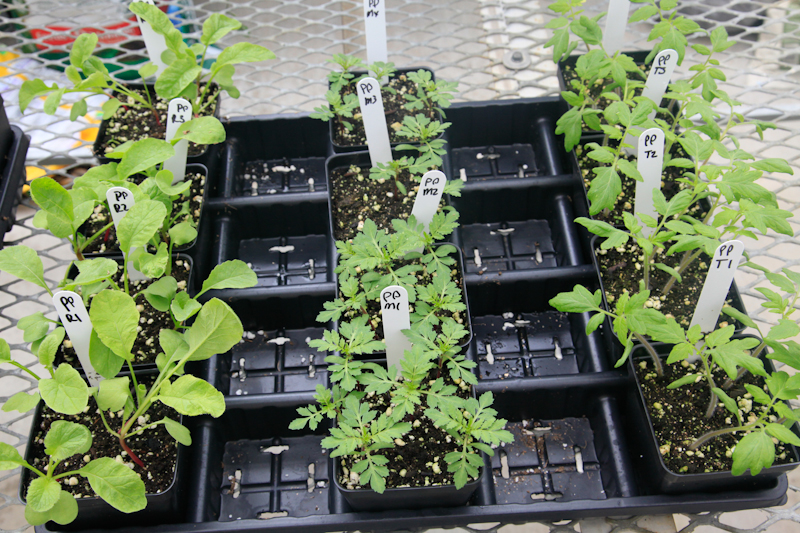
\includegraphics[width=0.9\textwidth]{Figure4_word.jpg}
  \caption{PP group potting arrangement during weeks 1 and 2 (germination phase). Photo taken at end of week 2. For scale, each pot is 8.9 cm x 8.9 cm x 6.1 cm (length x width x height)}
  \label{fig:pp}
\end{figure}

In a four week fertilizer experiment, Janie marigolds, Better Boy tomatoes, and Early Scarlet radishes were subjected to three different treatment types.  A control-control (CC) group was given control water (tap water) for the four-week duration.  A control-plasma (CP) group received control water for two weeks and then PAW for weeks 3 and 4; a plasma-plasma (PP) group received PAW throughout.  During the germination phase, weeks 1 and 2 of treatment, the plants were arranged as shown in \cref{fig:cc,fig:cp,fig:pp}.  Plant potting soil was composed of 60\% Canadian sphagnum peat, 20\% horticultural grade vermiculite, and 20\% horticultural grade perlite; all ingredients were blended together and brought to a moisture content of 50\% before potting.  A standard greenhouse environment was used with temperatures between 24 and 29 degrees Celsius during the day and between 16 and 21 degrees Celsius at night.  Additional experiments not discussed here indicate too much sunlight may negatively affect plant growth irrespective of water treatment type; consequently, shade curtains were used in the presented study to mitigate that effect.

At the end of the germination phase, a representative plant from each pot was chosen for treatment during the growth phase, weeks 3 and 4.  All other plants were removed from the pot.  This is exemplified by \cref{fig:cp_growth}.

\begin{figure}[htbp]
  \centering
  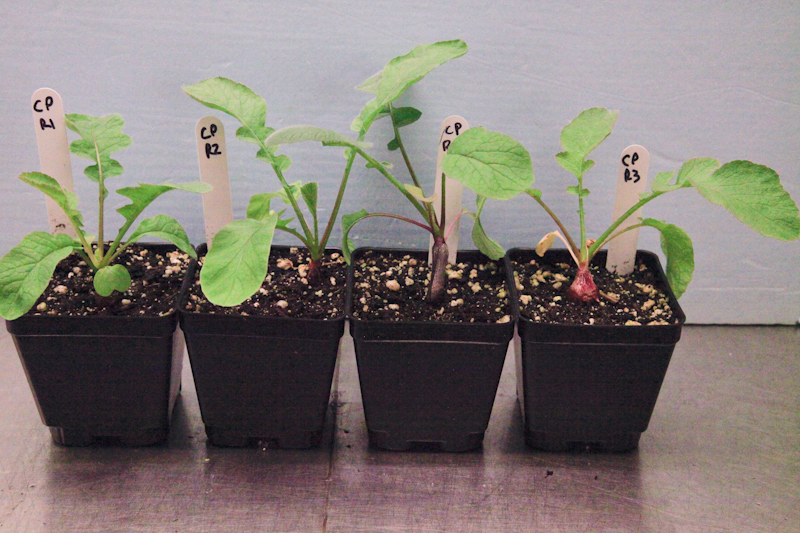
\includegraphics[width=0.9\textwidth]{Figure5_word.jpg}
  \caption{Potting arrangement during weeks 3 and 4 (growth phase) for CP group radishes.  A single representative plant from each pot was chosen at the end of the germination phase to continue on during the growth phase. For scale, each pot is 8.9 cm x 8.9 cm x 6.1 cm (length x width x height). Note that the 8.9 cm x 8.9 cm dimensions refer to the pot’s top as opposed to its base}
  \label{fig:cp_growth}
\end{figure}

During the germination phase, plants were misted 4-5 times per day; during the growth phase, plants received a traditional garden-style watering, e.g. steady water stream, 1-2 times per day.

\subsection{Results}

As explained in the experimental section, at the end of two weeks, a representative plant from each pot was chosen to continue into the growth phase.  At that time the height of the representative plants was recorded; this resulted in a sample size of eight plants for each control strain (radish, marigold, and tomato) and a sample size of four plants for each plasma strain (radish, marigold, and tomato).  The control sample size was twice as large as the plasma sample size because both CC and CP groups received tap water through the first two weeks.  The average height of these plants is shown in \cref{fig:germ_heights}. PAW treated plants showed a larger average height than their control treated counterparts; however, a two-tail Welch's t-test showed that none of the differences were statistically significant for a significance level of .05.  The t-test results are summarized in \cref{tab:germ_heights_t}.    The number of sprouted seedlings per pot was also counted and is presented in \cref{fig:germ_sprouts}.  Though the number of sprouted seedlings per pot was higher for control radishes and tomatoes compared to plasma groups, the differences were not statistically significant as indicated again by a two-tail Welch's t-test with a significance level of .05.  The t-test results for the number of sprouted plants per pot are summarized in \cref{tab:germ_sprouts_t}.

\begin{figure}[htbp]
  \centering
  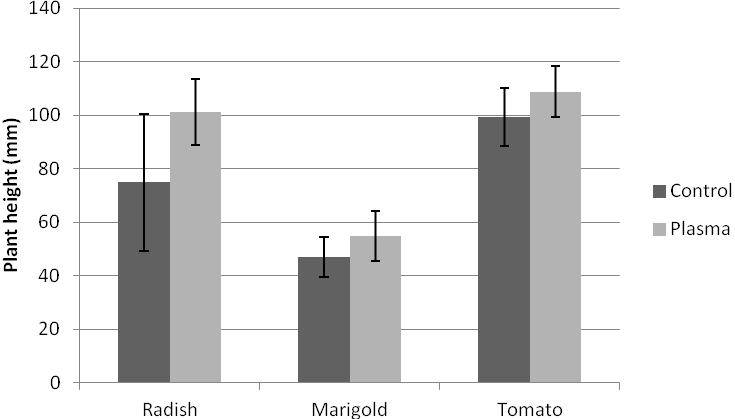
\includegraphics{Figure7_word.png}
  \caption{Comparison of control and plasma treated plant heights at end of germination phase (end of week 2) with accompanying error bars}
  \label{fig:germ_heights}
\end{figure}

\begin{table}[htpb]
  \begin{center}
    \begin{tabular}{c |c |c }
      Radish & Marigold & Tomato \\
      \hline
      .054 & .243 & .219
    \end{tabular}
  \end{center}
  \caption{Two-tail Welch's t-test results comparing control and plasma treated plants at end of germination phase.  Values shown are p-values}
  \label{tab:germ_heights_t}
\end{table}

\begin{figure}[htbp]
  \centering
  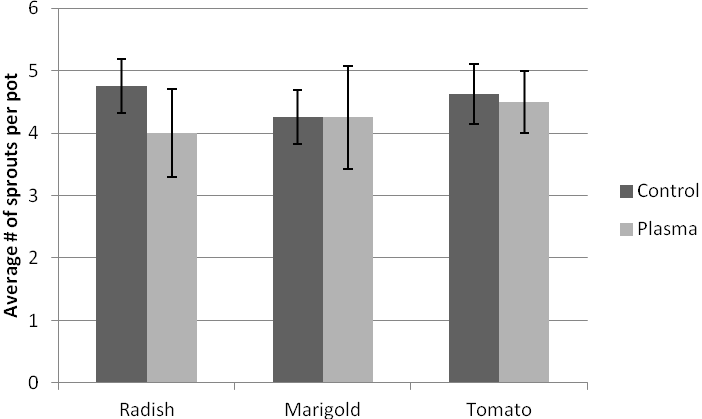
\includegraphics{Figure8_word.png}
  \caption{Comparison of control and plasma treated sprout data at end of germination phase (end of week 2) with accompanying error bars}
  \label{fig:germ_sprouts}
\end{figure}

\begin{table}[htpb]
  \begin{center}
    \begin{tabular}{c |c |c }
      Radish & Marigold & Tomato \\
      \hline
      .163 & 1 & .728
    \end{tabular}
  \end{center}
  \caption{Two-tail Welch's t-test results comparing the number of sprouted plants per pot for control and plasma treated plants at end of germination phase.  Values shown are p-values}
  \label{tab:germ_sprouts_t}
\end{table}

Beginning at the start of the growth phase, plant dimensions were measured almost daily. Because of practical difficulties with measuring the height, the distance spanned by the plants' true leaves was recorded.  Measurements are plotted in \cref{fig:radish_span,fig:marigold_span,fig:tomato_span}. Plants receiving PAW during this phase of the experiment, e.g. CP and PP groups, showed a marked improvement in growth relative to the CC group.

\begin{figure}[htbp]
  \centering
  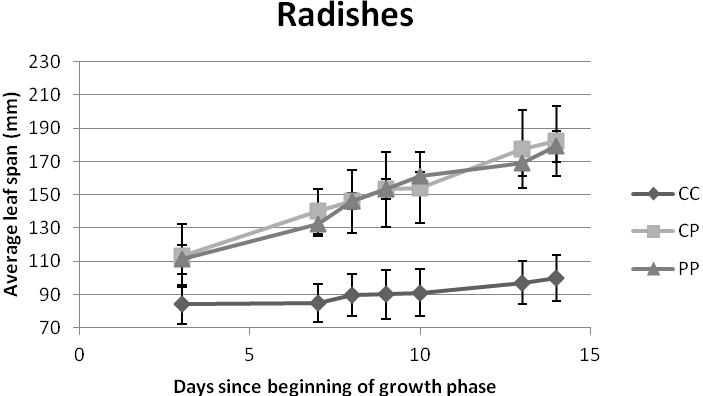
\includegraphics{Figure9_word.png}
  \caption{Average radish leaf span vs. time (growth phase, weeks 3 \& 4)}
  \label{fig:radish_span}
\end{figure}

\begin{figure}[htbp]
  \centering
  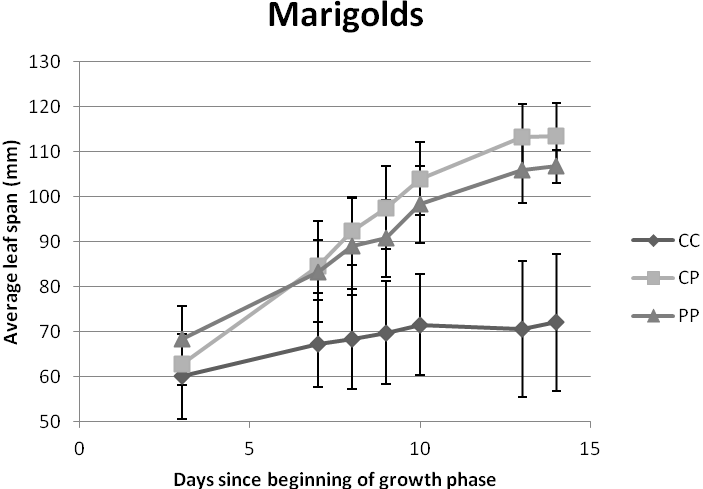
\includegraphics{Figure10_word.png}
  \caption{Average marigold leaf span vs. time (growth phase, weeks 3 \& 4)}
  \label{fig:marigold_span}
\end{figure}

\begin{figure}[htbp]
  \centering
  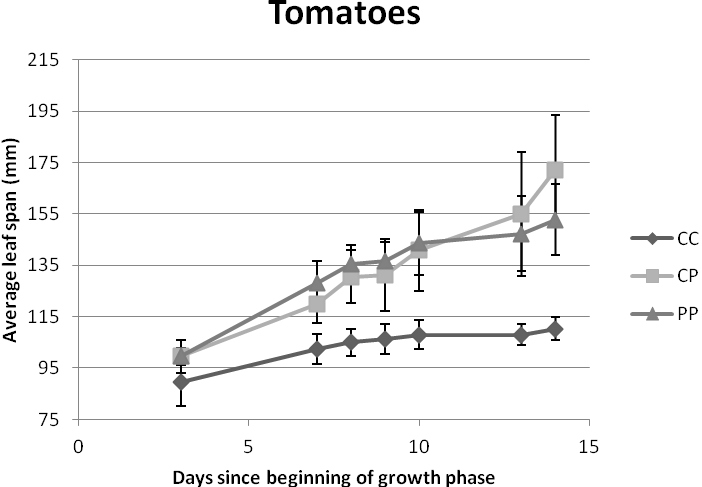
\includegraphics{Figure11_word.png}
  \caption{Average tomato leaf span vs. time (growth phase, weeks 3 \& 4)}
  \label{fig:tomato_span}
\end{figure}

In addition to the leaf span measurements recorded throughout the growth phase, photographs of representative plants were taken at the end of experiment in order to visually compare the relative sizes of the CC, CP, and PP groups.  These photos are shown in \cref{fig:radish_pic,fig:mari_pic,fig:tomato_pic}. CP and PP plants were larger in size than their CC counterparts.

\begin{figure}[htbp]
  \centering
  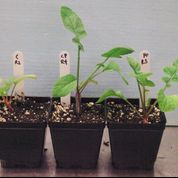
\includegraphics{Figure12_word.jpg}
  \caption{Representative radish plants at end of experiment. Left pot is CC; center is CP; right is PP}
  \label{fig:radish_pic}
\end{figure}

\begin{figure}[htbp]
  \centering
  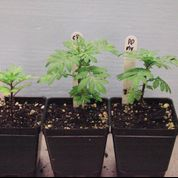
\includegraphics{Figure13_word.jpg}
  \caption{Representative marigold plants at end of experiment. Left pot is CC; center is CP; right is PP}
  \label{fig:mari_pic}
\end{figure}

\begin{figure}[htbp]
  \centering
  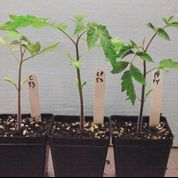
\includegraphics{Figure14_word.jpg}
  \caption{Representative tomato plants at end of experiment. Left pot is CC; center is CP; right is PP}
  \label{fig:tomato_pic}
\end{figure}

After the above photos were taken, plants were removed from their pots, washed, and dried.  Roots were separated from the above-ground plant called the shoot and both sections were weighed.  Average shoot and root dry weights are summarized in \cref{fig:shoots,fig:roots} respectively.  In agreement with \cref{fig:radish_pic,fig:mari_pic,fig:tomato_pic}, the average shoot masses of CP and PP plants were larger than CC plants.  A t-test, summarized in \cref{tab:shoot_t}, showed that all of these differences were statistically significant except for the difference between PP and CC marigolds (however, its test statistic of .06 was very close to our significance cut-off of .05).  In marigolds and tomatoes CP shoot masses were greater than PP shoots, however, the differences were within the error of the measurement.  Root mass results did not track with the shoot sizes and masses.  The root masses of CC radishes were on average larger than CP and PP radishes. CP marigold and tomato root masses were greater than their PP counterparts which were in turn larger than CC root masses.  However, all of the root mass differences were within the error of the measurement, and the t-test summarized in \cref{tab:root_t} indicates that the differences are not statistically significant.

\begin{figure}[htbp]
  \centering
  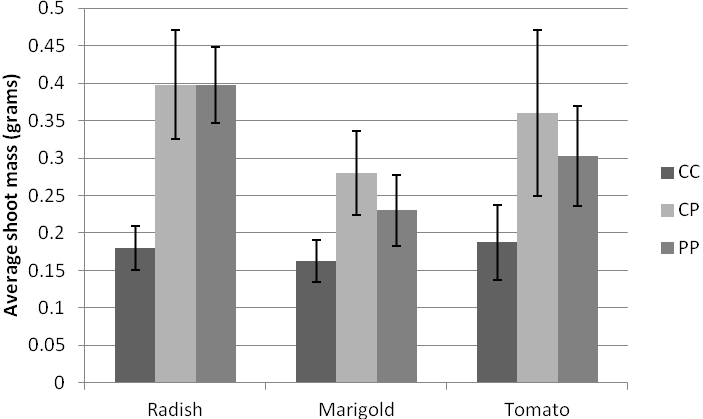
\includegraphics{Figure15_word.png}
  \caption{Average shoot dry mass by plant and treatment types at end of experiment}
  \label{fig:shoots}
\end{figure}

\begin{figure}[htbp]
  \centering
  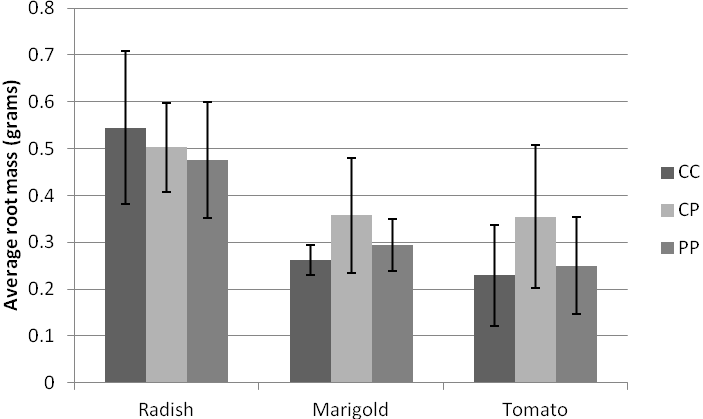
\includegraphics{Figure16_word.png}
  \caption{Average root dry mass by plant and treatment types at end of experiment}
  \label{fig:roots}
\end{figure}

\begin{table}[htpb]
  \begin{center}
    \begin{tabular}{|l |c |c |c |}
      \hline
      Shoot Mass & PP vs. CP & PP vs. CC & CP vs. CC \\\hline
      Radish & 1.000 & 0.001 & 0.005 \\\hline
      Marigold & 0.224 & 0.060 & 0.017 \\\hline
      Tomato & 0.414 & 0.035 & 0.044 \\\hline
    \end{tabular}
  \end{center}
  \caption{p-values for comparisons between the shoot masses of different plans and treatment groups. Values below .05 indicate a statistically significant difference between the species being compared}
  \label{tab:shoot_t}
\end{table}

\begin{table}[htpb]
  \begin{center}
    \begin{tabular}{|l |c |c |c |}
      \hline
      Root Mass & PP vs. CP & PP vs. CC & CP vs. CC \\\hline
      Radish & 0.738 & 0.523 & 0.674 \\\hline
      Marigold & 0.402 & 0.360 & 0.218 \\\hline
      Tomato & 0.304 & 0.798 & 0.235 \\\hline
    \end{tabular}
  \end{center}
  \caption{p-values for comparisons between the root masses of different plans and treatment groups. Values below .05 indicate a statistically significant difference between the species being compared}
  \label{tab:root_t}
\end{table}

\subsection{Discussion}

Over the course of a four week experiment plants which received PAW in weeks 3 and 4 (CP group) and plants which received PAW for all four weeks (PP group) grew significantly larger than tap water controls (CC group).  Differences between PAW and control groups did not emerge immediately.  As shown in \cref{fig:germ_heights} and by the statistical analysis in \cref{tab:germ_heights_t}, control and plasma treated plants were not significantly different in size after two weeks.  It should also be noted from \cref{fig:germ_sprouts} and \cref{tab:germ_sprouts_t} that PAW and control groups did not show significant differences in germination rates.  However, during the growth phase, weeks 3 and 4, differences between PAW treated plants and tap water controls became evident.  In \cref{fig:radish_span,fig:marigold_span,fig:tomato_span} the increased growth rate of CP and PP plants relative to CC is evident in the sizable slope differences.  The side-to-side photographs in \cref{fig:radish_pic,fig:mari_pic,fig:tomato_pic} show the greater height and foliage of CP and PP plants compared to their CC counterpart.  Moreover, although it is difficult to note in the photographs, CP and PP plants had a healthy, green color at the end of the 4-week experiment; CC plants had begun to yellow and wither.  \Cref{fig:shoots,fig:roots} compare the root and shoot masses for different treatment groups.  \Cref{tab:shoot_t,tab:root_t} show p-values indicating the level of difference in shoot and root masses between groups.  Smaller p-values indicate larger statistical differences; a value of .05 has been chosen as the threshold level to indicate significant statistical differences.  Using that significance level, it is found that CP plants all had significantly larger shoot masses than tap water controls.  PP radishes and tomatoes were significantly larger than controls; PP marigolds were not significantly different from control marigolds (although the p-value of .06 is close to the threshold for significance).  There were not any significant differences between CP and PP shoot masses.  The differences found in shoot masses were not reflected in the root mass data.  \Cref{tab:root_t} shows that no groups demonstrated significant differences in root mass.   The general increase in shoot mass of PAW treated plants is believed to occur primarily because of the nitrate present in PAW after plasma exposure.  Nitrogen is well known to be an essential plant nutrient, necessary for proteins, enzymes, and metabolic processes; ion chromatograph and Total N analyses reveal that nitrite and nitrate are the long-lived nitrogen species in PAW.  Moreover, nitrate concentrations are a factor of 20 larger than nitrite concentrations in these plant experiments and so should be the dominant nitrogen specie that the plants are exposed to.

\section{Remediation of Aqueous Pollutants}
\label{sec:pollutant}

As discussed in \cref{chap:intro}, plasmas in contact with liquids produce a cornucopia of reactive species, including both highly oxidative species like OH and highly reductive species like e$^-$. There is considerable interest in the low-temperature plasma community in using these highly reactive species to degrade persistent chemicals in waste streams, both gaseous and liquid. Below, we explore using the VHF atmospheric source to degrade dioxane, a known carcinogen, and perfluorooctanesulfonic acid (PFOS) which has been associated with increased risk of chronic kidney disease. \cite{shankar2011perfluoroalkyl}

\subsection{Dioxane}
\label{sec:dioxane}

In an experiment to test the efficacy of plasma for treating dioxane, a 500 mL solution of 400 $\mu$g/L dioxane was treated for 26 minutes with a 420 W air discharge using the geometric configuration shown in \cref{fig:batch_scheme}. The time profile of dioxane concentration is shown in \cref{fig:diox_compare_argon_air}; it follows a simple exponential decay shape. After 26 minutes, 98\% of the dioxane has been removed. This compares very favorably to an AOT study in the literature (\cite{suh2004study}). In the literature study, the treated solution was a factor of two larger; however, the concentration of dioxane was two to three orders of magnitude higher. The plasma decadal treatment time was slightly shorter than the literature study's.

\begin{figure}[htbp]
  \centering
  \includegraphics{air_plasma_treating_dioxane.png}
  \caption{Photograph of 420 W ``calm'' air discharge treating aqueous dioxane solution.}
  \label{fig:diox_air}
\end{figure}

\begin{figure}[htbp]
  \centering
  \includegraphics[width=0.9\textwidth]{argon_plasma_treating_dioxane.png}
  \caption{Photograph of 350 W ``bright'' argon discharge treating aqueous dioxane solution}
  \label{fig:diox_argon}
\end{figure}

A 350 W argon discharge was also used in the dioxane treatment study. Even at a lower power relative to the air discharge, no dioxane was detected after 5 minutes of treatment. This result can be seen in \cref{fig:diox_compare_argon_air}. The near order of magnitude better performance of argon over air discharge is interesting. Some feeling of the fundamental difference in performance can be gleaned by looking at the appearance of the discharges. The calm air discharge can be seen in \cref{fig:diox_air}; the much brighter and much larger surface area argon discharge can be seen in \cref{fig:diox_argon}. The bright blue color in the argon discharge is likely due to plasma interactions with the aluminum electrode. It is conceivable that the plasma-metal interactions create a larger density of electrons in the discharge that in turn lead to greater creation of oxidative species like OH from water vapor and/or the ambient air. Or it is possible that the greater density in gas phase electrons translates into a greater density of hydrated electrons and that degradation of dioxane may proceed through a reductive pathway as opposed to an oxidative one. Such uncertainty in reaction mechanisms is one of the fundamental reasons that the modelling work described in \cref{chap:basic_science} was begun; until experimental diagnostics are developed that are capable of detailed and comprehensive probing of both gas and near-inteface liquid chemistry, models are a good way to qualitatively explore the plasma-liquid dynamics.

Despite its rapid success in treating dioxane, there are several drawbacks to using the argon discharge. One is that argon is much more expensive than air; for treatment plant wastewater scales, the cost is likely to be prohibitive. Another problem is the erosion of the metal electrode; this could be alleviated by using the pure water electrode configruation (see \cref{fig:water_electrode_scheme,fig:water_electrodes_image}). However, removal of the argon-metal interaction could very well decrease the efficacy of the argon-dioxane treatment. A final problem with the argon discharge is its transient nature. When operating the argon discharge, the load impedance can oscillate wildly. This makes impedance matching very difficult, leading to lots of reflected power to the generator. Despite these issues, the argon treatment result is intriguing because of its considerably greater efficacy when compared to leading AOTs like H$_2$O$_2$/O$_3$. Moreover, the air-dioxane treatment, which lacks the issues associated with the argon treatment, also compares reasonably well to the H$_2$O$_2$/O$_3$ method. Finally, as illustrated by the PFOS results presented in \cref{sec:PFOS}, the \cref{fig:batch_scheme} configuration is unlikely to be the best scheme for maximizing plasma-liquid interactions and destroying persistent chemicals. The configuration presented in \cref{fig:water_electrode_scheme} is likely a better choice; indeed a preliminary experiment showed a one-pass reduction in the concentration of dioxane from 365 $\mu$g/L to 172 $\mu$g/L using the pure water electrode design.

\begin{figure}[htbp]
  \centering
  \includegraphics{argon_vs_air_dioxane.png}
  \caption{Comparison of argon and air discharges for removing dioxane from solution}
  \label{fig:diox_compare_argon_air}
\end{figure}

\subsection{PFOS}
\label{sec:PFOS}

 When PFOS solution is treated using the geometric configuration shown in \cref{fig:batch_scheme}, no degradation is observed.  However, when PFOS solution is treated using the pure water electrode geometry of \cref{fig:water_electrode_scheme}, degradation is observed. Experimental conditions are 700 W delivered to the plasma, 3 standard cubic meet per minute of air flow, and a roughly 50 $\mu$g/L starting concentration of PFOS. PFOS concentrations are measured using a high performance liquid chromatography (HPLC) instrument provided by the Environmental Protection Agency. The time vs. PFOS concentration profile is shown in \cref{fig:PFOS_degradation}. The curve shows an exponential decay shape that appears to level around a concentration of 5 $\mu$g/L. Ninety percent reduction in PFOS concentration is considered a significant success by colleagues at the EPA. Additional work has focused on trying to elucidate the PFOS degradation mechanism by examining degradation products; however, measurements with HPLC/TOF-MS, ion chromatography, and other methods have been inconclusive. Thus, it is unknown whether PFOS breaks down via oxidative or reductive routes. That the batch treatment scheme is totally unsuccessful in achieving degradation suggests a reductive route since the OH radical concentrations are not expected to vary significantly between \cref{fig:batch_scheme} and \cref{fig:water_electrode_scheme} while the charged particle fluxes, including electrons, are expected to be much larger in the latter case. However, new experimental techniques or detailed models will be required to confirm that hypothesis. This is again motivation for the work that is started in \cref{chap:basic_science}.

\begin{figure}[htbp]
  \centering
  \includegraphics[width=0.9\textwidth]{PFOS_degradation.png}
  \caption{PFOS concentration vs. treatment time using the water electrode}
  \label{fig:PFOS_degradation}
\end{figure}

\section{Summary}

This chapter investigates a couple applications of plasma-liquids. \Cref{sec:fertigation} explores fertilization of radishes, tomatoes, and marigolds indirectly through plasmas. PAW treated plants are shown to grow 1.7-2.2 times larger than their tap-watered peers because of the aqueous NO$_x$ species dissolved into solution by the plasma. \Cref{sec:pollutant} describes remediation of aqueous contaminants using the VHF source. The batch configuration using air as the feed gas is shown to be effective at removing 1,4-dioxane. However, replacing air with argon leads to an order of magnitude improvement in dioxane removal. While the batch configuration is unable to degrade PFOS, the water electrode geometry is capable of removing the contaminant. Improvement of pollutant removal rates will rely on increased understanding of the reaction mechanism and dissolution of reactive plasma species. This is a logical extension of the modelling work in \cref{chap:basic_science,chap:zapdos} and experimental characterization in \cref{chap:expt_opt}. Concluding thoughts on intertwining modeling and experimental efforts in the broader scope of plasma-liquid science are contained in the final chapter of the dissertation, \cref{chap:conclusion}.
